\documentclass[english]{article}
\usepackage[T1]{fontenc}
\usepackage[latin9]{inputenc}
\usepackage{geometry}
\geometry{verbose,tmargin=3cm,bmargin=3cm,lmargin=3cm,rmargin=3cm}

\makeatletter
\usepackage{url}

\makeatother

\usepackage{babel}
\usepackage{xcolor}
\usepackage[backend=bibtex, style=ieee]{biblatex}
\addbibresource{bibliography.bib}
\usepackage[hidelinks]{hyperref}
\usepackage{graphicx}
\graphicspath{ {./images/} }

\title{Draft Research Plan for Multi-Agent Path Finding with Matching using A* with OD and ID}
\author{Ivar de Bruin}
\date{\today}

\newcommand{\namelistlabel}[1]{\mbox{#1}\hfil}
\newenvironment{namelist}[1]{%1
\begin{list}{}
    {
        \let\makelabel\namelistlabel
        \settowidth{\labelwidth}{#1}
        \setlength{\leftmargin}{1.1\labelwidth}
    }
  }{%1
\end{list}}

\begin{document}
\maketitle

\begin{namelist}{xxxxxxxxxxxxxxxxxxxxxxxxxxxxxxxxxxxxxxx}
\item[{\bf Title:}]
	Multi-Agent Path Finding with Matching using A* with OD and ID
\item[{\bf Author:}]
	Ivar de Bruin
\item[{\bf Responsible Professor:}]
	Mathijs de Weerdt
%\item[{\bf (Required for final version) Examiner:}]
%	Another Professor (\emph{interested, but not involved})
\item[{\bf Peer group members:}]
	Robbin Baauw, Jonathan D\"onszelmann, Jaap de Jong, Thom van der Woude
\end{namelist}


\section*{Background of the research}
The Dutch Railways (NS) is tasked with maintaining trains during the night. 
The trains are routed to shunting yards where they can be cleaned and receive maintenance. 
Here there is an NP-hard problem called the Train Unit Shunting and Servicing (TUSS) problem. 
One of the main questions in this problems is with regards to the capacity of these shunting yards. 
To try and establish an upper bound to this capacity we try to find a relaxation to the problem. 

The NP-hard Multi-Agent Path Finding (MAPF) describes multiple agents on a graph, moving from a start node to a goal node while avoiding collisions. 
In this problem we try to minimize the sum of individual costs (SIC).
To make this problem into a relaxation of the TUSS problem we also need to introduce matching, as there is no exact assignment per train for a destination but rather per class or type of train.
\\\\%TODO: describe current state
{\color{red}Description of current state of the research field to be added later}


\section*{Research Question}
The main question that will be answered in this paper is: How can the MAPF algorithm A* with ID and OD be used to solve a relaxation of the TUSS problem when it is expanded with matching. We can then look at the following sub-questions:
\begin{itemize}
	\item Which matching algorithm performs best when combined with A* with OD and ID
	\item How does this combined algorithm perform compared to other MAPF algorithms expanded with matching?
	\item Under which conditions should this algorithm be used?
	\item Under which conditions should this algorithm not be used?
\end{itemize}
%TODO: Fix and expand
{\color{red}Will be expanded and improved later this week}

\section*{Method}
%TODO: describe method
{\color{red}Method explanation will be added later this week}

\section*{Planning of the research project}
\subsection*{Task description: Orientation}
The first week will be spent on orientation. What is the current state of the field?  How does A* ID OD really work. How can I make it? etc.
\\\\
During this week I will also orientate myself on the different deadlines and lectures we have. For example how to prepare for each one.
\\\\
For this orientation I will also be reading quite a few papers starting with Standley's paper on A* with ID and OD \cite{AStarIDOD_standley_2010}, Stern et al. paper on Multi-Agent pathfinding\cite{stern2019multiagent} and Mulderij et al. paper on the TUSS problem\cite{mulderij2020train}. As well as any papers that follow from that that seem relevant.
\\\\
This orientation should then finally allow me to make the final version of this research plan at the end of the week.
%TODO: create planning
{\color{red}Rest of planning will be added later this week}
\subsection*{Planning overview}
\begin{figure}[h]
	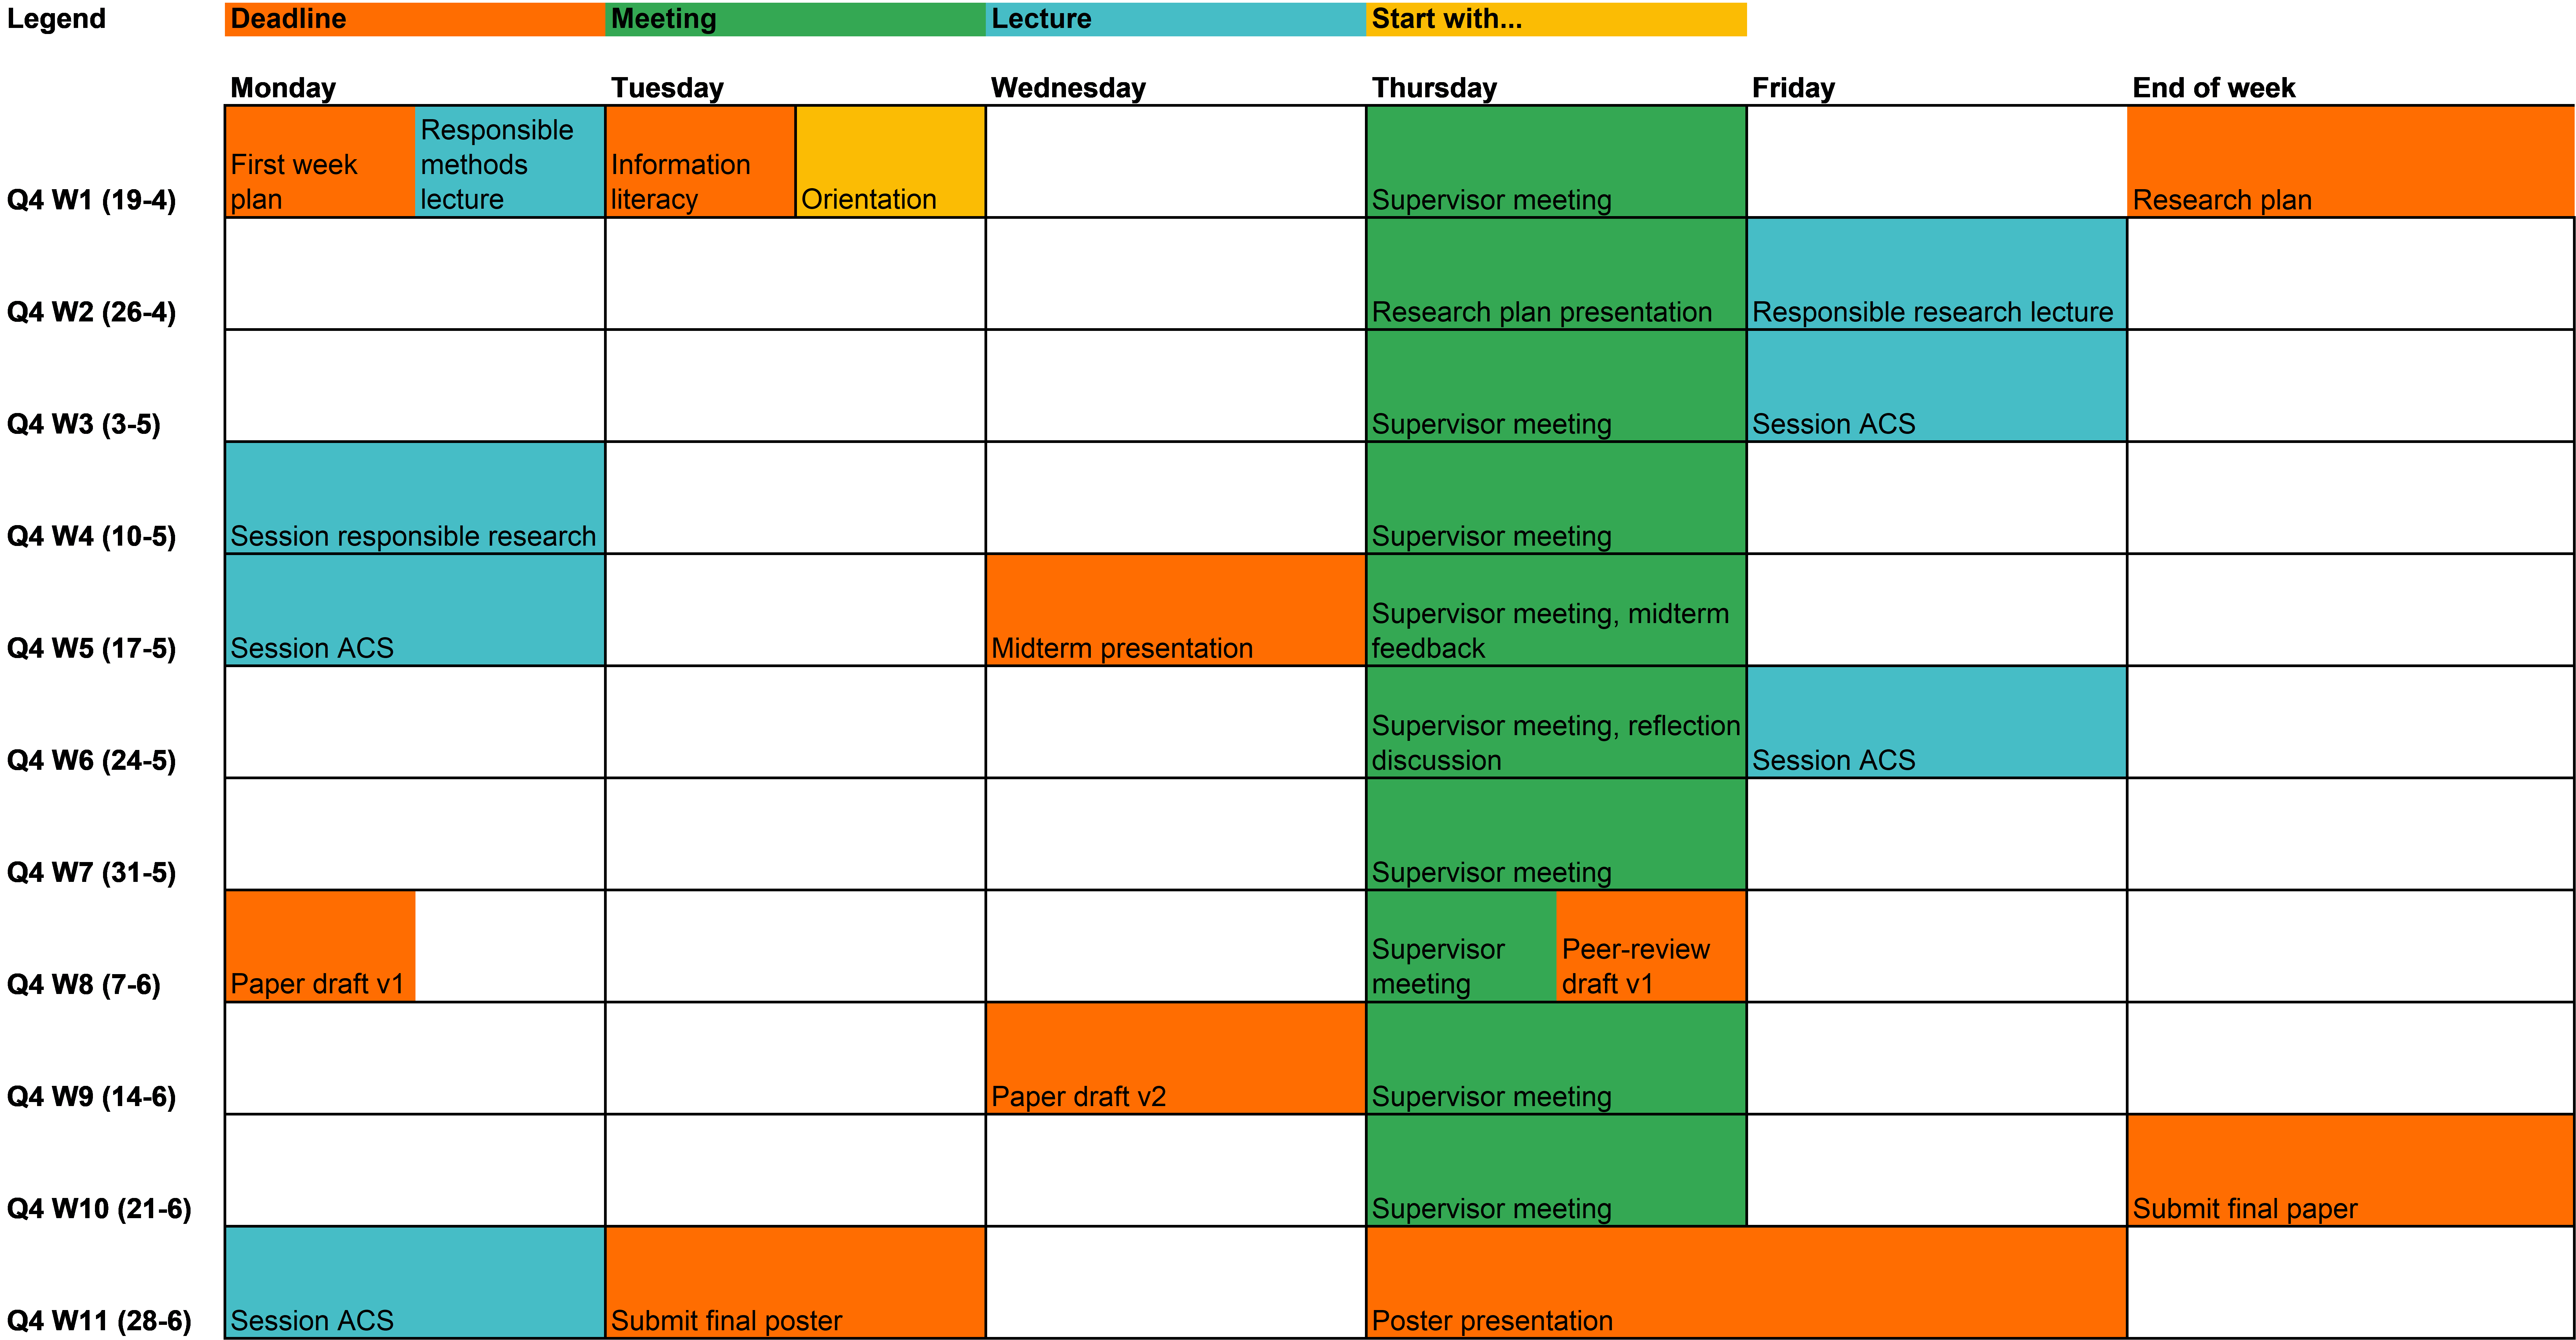
\includegraphics[width=\linewidth]{Planning}
	\centering
	\caption{Draft planning overview}
\end{figure}


\pagebreak
\printbibliography

%for convenience we use here the in-document bibliography
%\begin{thebibliography}{9}
%\bibitem{wessen} Ken Wessen, Preparing a thesis using \LaTeX~, private
%communication, 1994.
%\end{thebibliography}

\end{document}
